%% LyX 2.3.2-2 created this file.  For more info, see http://www.lyx.org/.
%% Do not edit unless you really know what you are doing.
\documentclass[english]{revtex4-1}
\usepackage[T1]{fontenc}
\usepackage[latin9]{inputenc}
\setcounter{secnumdepth}{3}
\usepackage{float}
\usepackage{graphicx}
\usepackage{babel}

\begin{document}
\title{Prelim document draft.}

\maketitle
Central Questions:  By making an Al/Na$_{3}$Bi heterostructure, can we make topological states?

\section{Introduce Topological Insulators and Topological Dirac Semimetals.}

Topological materials have garnered significant attention in the condensed matter community in past few years because of their peculiar electronic properties exhibited in the weakly and strongly interacting types. Here we will focus on the uncorrelated topological systems, in particular topological insulators and semimetals. Topological insulators feature a insulating (or gapped band spectrum) in their bulk but are conducting (or gapless) on the surface that encloses the bulk. The gapless states on their surfaces are termed chiral currents, which are characterized by spin-momentum locking. Effectively, the propagation direction of the charge carriers is set by their spin degree of freedom. Moreover, at energies and momenta near the surface band crossing points in these systems, the dispersion attains a form of a non-relativistic version of a massless Dirac dispersion relation. Overall, topological insulators like $BiSe_3$ have a crucial symmetry known as time-reversal symmetry, which prevents the chiral surface states from being gapped.

Since then, new materials which feature both a gapless bulk and surface states have been discovered theoretically and experimentally. These materials are known as topological semimetals. There are a variety of topological semimetals like Weyl,Dirac, and nodal line semimetals, just to name a few.  We will look at Weyl and Dirac semimetals because they share a number of common traits, but also important differences. Part of this is based on the type of degeneracies in the band plots. We will provide a short explanation about their differences.

In a band structure plot of the energy states there are cases where bands corresponding to different energy eigenvalues can be degenerate from accidental degeneracies (i.e. from tuning parameters in the Hamiltonian such that two or more energy levels can have the same energy). The presence of symmetries can increase the degeneracy of the band crossing points. (There are symmetries that can induce band crossings?) Most of the 3-D semimetals have time reversal and inversion symmetries. Inversion symmetry reverses the sign of the momentum, but not the spin of the particular band:

\begin{equation}
E_{n,\sigma}\left({\bf k}\right)=E_{n,\sigma}\left(-{\bf k}\right).
\end{equation}

\noindent Time reversal symmetry reverses both the spin of the particular band and the sign of the momentum:

\begin{equation}
E_{n,\uparrow}\left({\bf k}\right)=E_{n,\downarrow}\left(-{\bf k}\right).
\end{equation}

\noindent If both time-reversal symmetry and inversion symmetry are present, then:

\begin{equation}
E_{n,\uparrow}\left({\bf k}\right)=E_{n,\downarrow}\left({\bf k}\right),
\end{equation}

\noindent which indicates that there is a double degeneracy for bands of different spin components at each k-point. If there is a degeneracy of bands, at some momentum ${\bf k}_{0}$, of different quantum number $n$,
say $n$ and $n+1$, then that band crossing point is four-fold degenerate.
If we expand the Hamiltonian at the band crossing point and if this
gives a massless Dirac dispersion relation, then this band crossing
point can be regarded as an emergent and non-relativistic Dirac particle.
In the case where there is a breaking of time-reversal symmetry, or
inversion-symmetry, or both, the double degeneracy of the a single
band is lifted over generic points in the Brillouin zone. In this
case, when two such bands meet at the same energy at some momentum
in the Brillouin zone, there is a degeneracy of two. If one expands
the Hamiltonian around the momentum crossing point of the two bands,
and if one finds a relativistic Weyl dispersion, such band crossings
are called Weyl nodes. Each Weyl node carries a non-zero ``charge''
which is computed by integrating the Berry curvature around a small
closed surface $S$ that encloses the Weyl node.  This is defined as the Chern number:

\begin{eqnarray}
C = \frac{1}{2\pi} \sum_{n=1}^{n=N} \oint_S \vec{\Omega}_{n}(\text{k}) \cdot d\vec{S}_{\vec{k}}\\
\vec{\Omega}_{n}(\bf{k}) = \nabla_{\bf{k}} \times \langle u_n(\bf{k}) | -i \nabla_{\bf{k}} |u_n(\bf{k})\rangle
\end{eqnarray}

\noindent Here we assume there are $N$ filled bands.   

Weyl semimetals have a bulk momentum space that is characterized by an even number of band crossing points where two non-degenerate bands meet. The total Chern number of all the Weyl points in the bulk momentum space is zero, which indicates that there are equal number of Weyl points with opposite Chern number in the bulk Brillouin zone.  These degeneracies are stable so long as they remain in different momentum space points.  If the Weyl points of opposite Chern number coincide in momentum space, the degenercy of the two states is lifted (it  becomes gapped).  The degeneracies in the bulk momentum space of the Weyl semimetal have interesting surface states that appear on the surface Brillouin zone of the Weyl semimetal. These surface states are known as Fermi arcs which are incomplete Fermi surfaces that connect the surface projections of the bulk Weyl points.

For Dirac semimetals the Dirac point is a four-fold degenerate point in momentum space.  This point contains two Weyl points of opposite Chern number, which give the Dirac point a vanishing Chern number. Certain symmetries are needed required in order for the Dirac point to remain stable at the same momentum space point. At first, the existence of a Dirac semimetal was thought to exist at the phase boundary between a topological insulator and a conventional insulator, as long as time reversal and inversion symmetry were preserved, thereby giving a four-fold degenerate bulk band crossing at the phase boundary.  (cite TSMs from 1st principles).  However, there have since been other realizations of topological Dirac semimetals.   



\begin{itemize}
    \item What is exciting people about heterostructures comprised of topological materials, such as Bismuth Selenide?  Clearly the strong spin-orbit coupling present in such materials is one interesting aspect that can be harnessed in heterostructures.
    \item Topological Dirac semimetals can have strong spin-orbit coupling.  
\end{itemize}



\section{Some of our data.}

%Baseline system: Na3Bi topological Dirac semimetal.
\begin{itemize}
    \item We looked at the surface states of the topological Dirac semimetal Na$_{3}$Bi at the surface along the (110) direction, or more accurately the (11$\bar{2}$0) direction.
    \item The reason why we chose this direction was because this surface is parallel to the $k_{z}$ axis along which there are two Dirac point crossings (cite Na3Bi 2012 paper).
    \item It is believed the Fermi arc surface states appear on this surface for $k_{z}=0$ since that $z$-component of momentum is time-reversal symmetric. (cite PNAS paper).

\end{itemize}


%Na3Bi band gap oscillations.
\subsection{Na$_{3}$Bi (110) slab and vacuum thickness effects on Na$_{3}$Bi's band structure.}

\begin{figure}[H]
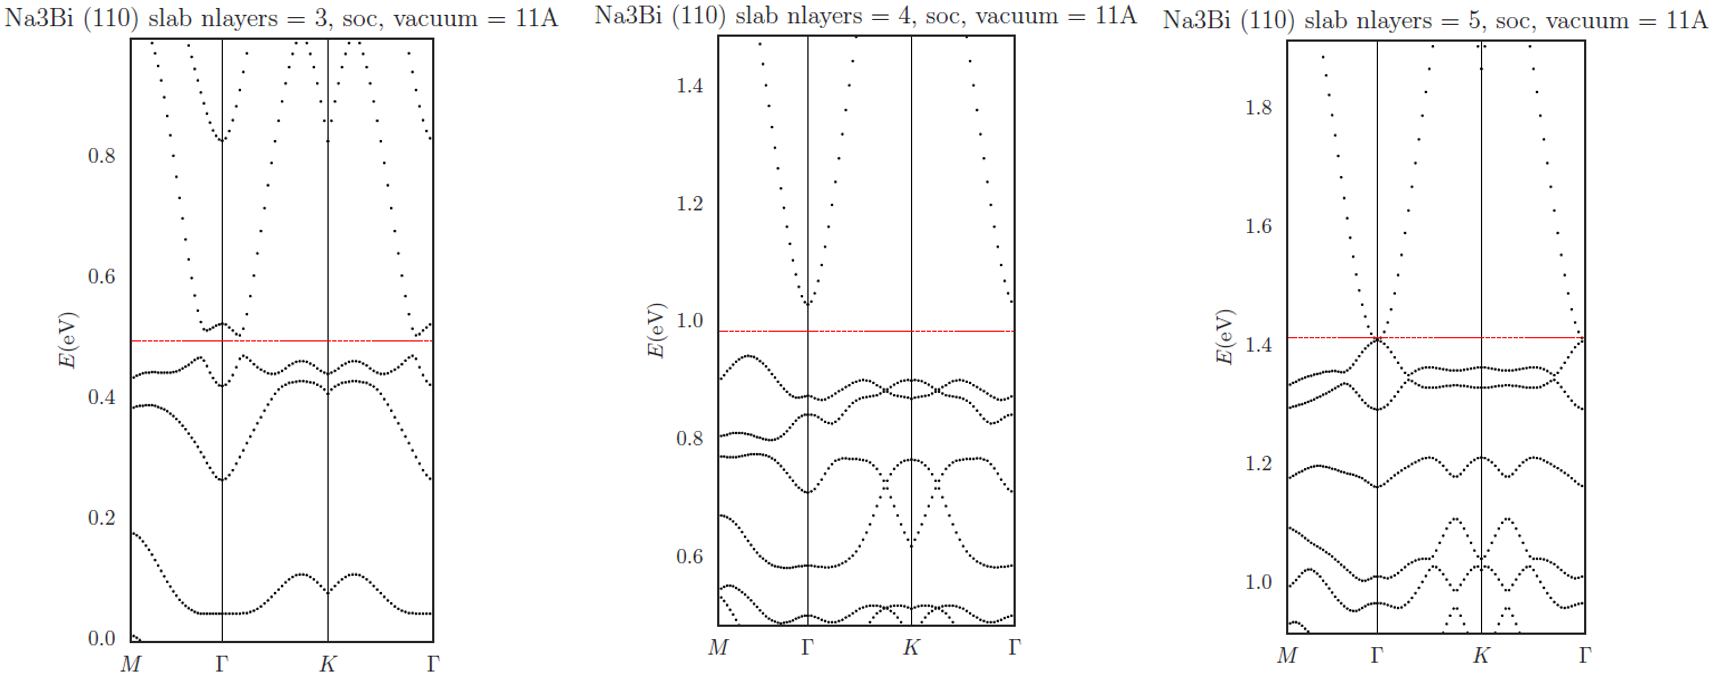
\includegraphics[scale=0.62]{Na3Bi_change_nlayers_vac_11A}\caption{\label{fig:Band-plots-of Na3Bi changing thickness}Band plots of the
Na$_{3}$Bi (110) system with fixed vacuum thickness but varying system thickness. The red line is the Fermi level.}
\end{figure}

\begin{itemize}
    \item We see in Figure \ref{fig:Band-plots-of Na3Bi changing thickness} that as the number of Na$_{3}$Bi layers increases, the band gap size at the $\Gamma$ point oscillates, with odd layers having a smaller band gap than even layers.  
    \item This is consistent with the oscillatory decay of Na$_{3}$Bi's band gap when the confining direction (i.e. the direction with open boundary conditions) is along the z-direction.
    \item Why are we interested in the $\Gamma$ point? It is perhaps because at that momentum, the band inversion is most visible. We see hints of the band inversion for the 3 layer Na$_{3}$Bi (110) structure above at the $\Gamma$ point, for the conduction and valence bands nearest the Fermi level.
\end{itemize}

\begin{figure}[H]
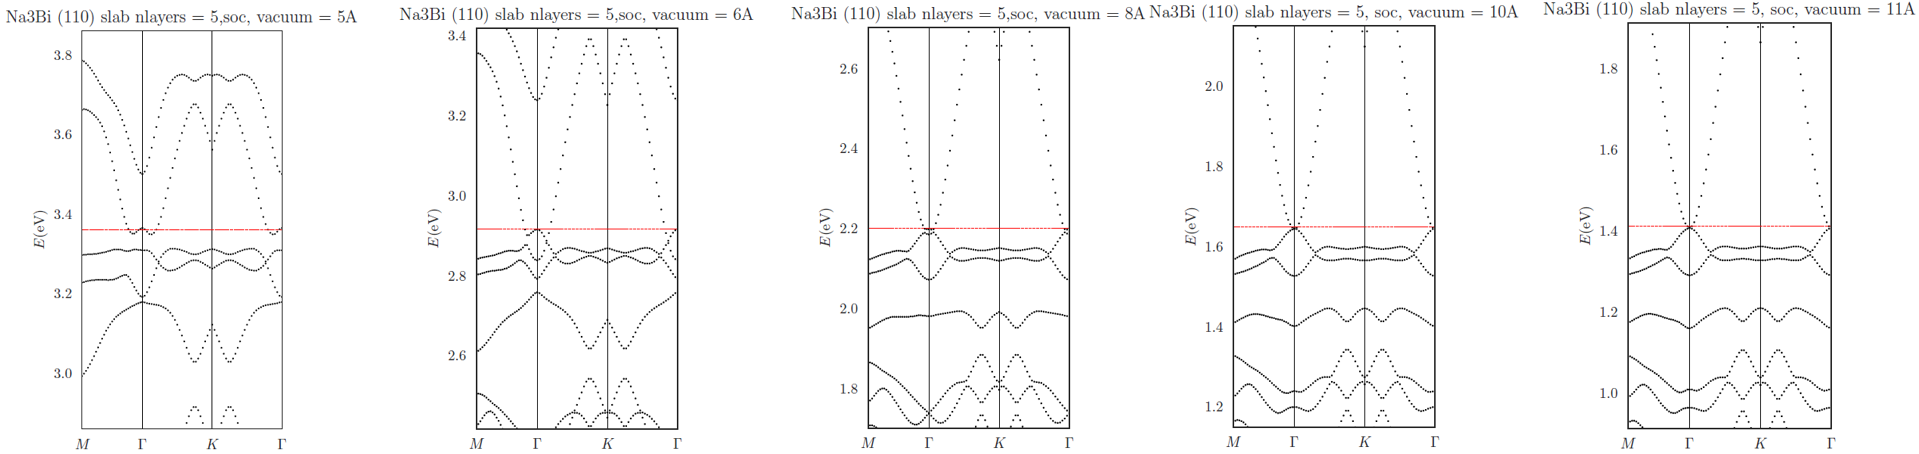
\includegraphics[scale=0.6]{Na3Bi_nlayer_5_change_vac}\caption{\label{fig:Na3Bi Fixed odd number layers incr vac}Band plots for a variable vacuum thickness surrounding a 5 layer Na$_3$Bi structure.}
\end{figure}

\begin{itemize}

    \item Figure \ref{fig:Na3Bi Fixed odd number layers incr vac} summarizes how changing the vacuum thickness affects the band plots of a 5 layer Na$_3$Bi system. We find hints of band inversion for bands nearest the Fermi level at the $\Gamma$ point for the system surrounded by an 8A vacuum layer. 
    \item Overall the band plots demonstrate little to no band gaps around the Fermi level near the $\Gamma$ point.
\end{itemize}


\begin{figure}[H]
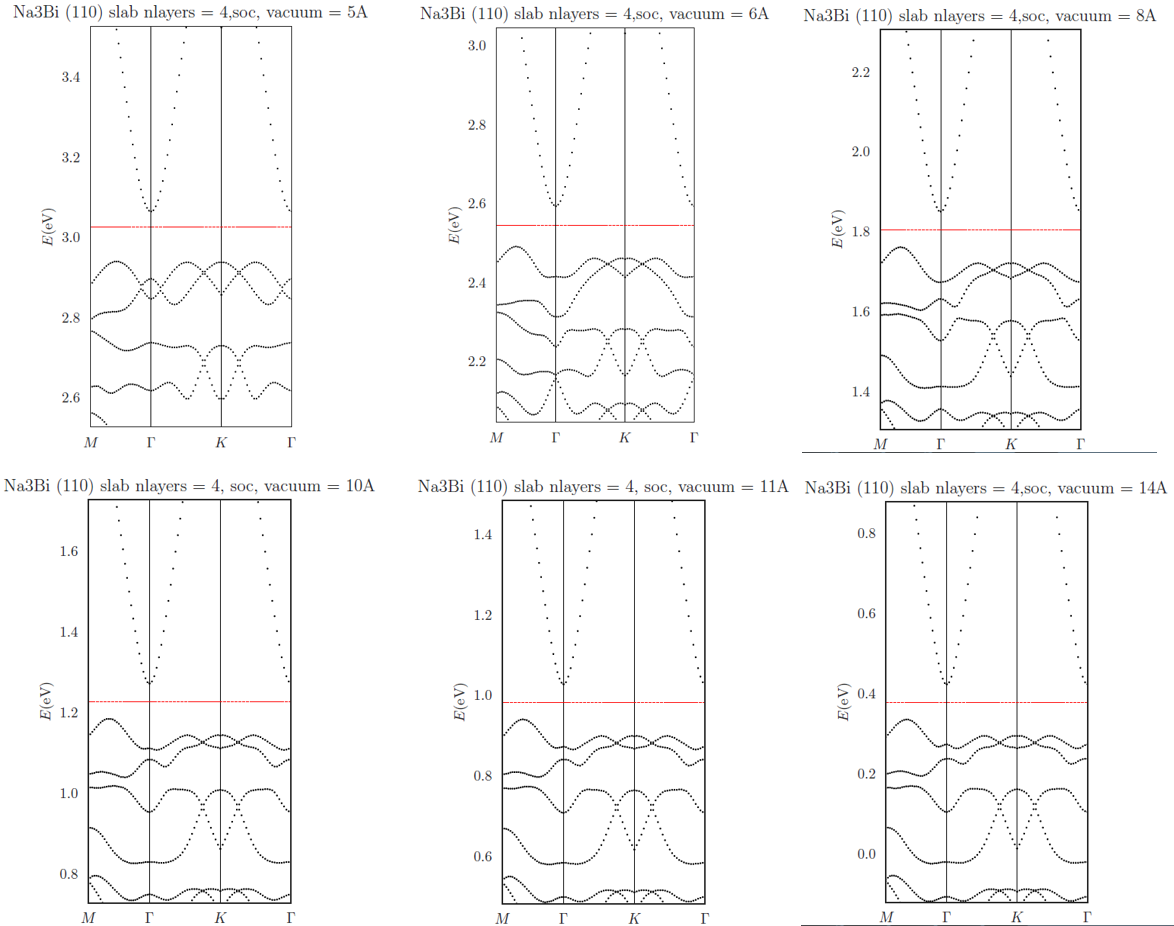
\includegraphics[scale=0.65]{Na3Bi_nlayer4_change_vac}

\caption{\label{fig:Na3Bi Fixed even number layers incr vac} Band plots for a variable vacuum thickness surrounding a 4 layer Na$_3$Bi structure.}
\end{figure}

\begin{itemize}

    \item If we compare Figure \ref{fig:Na3Bi Fixed even number layers incr vac} with Figure \ref{fig:Na3Bi Fixed odd number layers incr vac} we observe a larger band gap in the former than the latter for similar vacuum thicknesses.
    \item There does not appear to be any band inversion in the character of the bands nearest to the Fermi level at the $\Gamma$ point. 
    \item Overall, we need to find the Berry curvature of these systems in order to definitively determine their topological characteristics.
\end{itemize}



%Fat band calculations for plain Na3Bi.
\subsection{Contributions of Na and Bi atom orbitals to the Na$_{3}$Bi band plots.}

\begin{figure}[H]
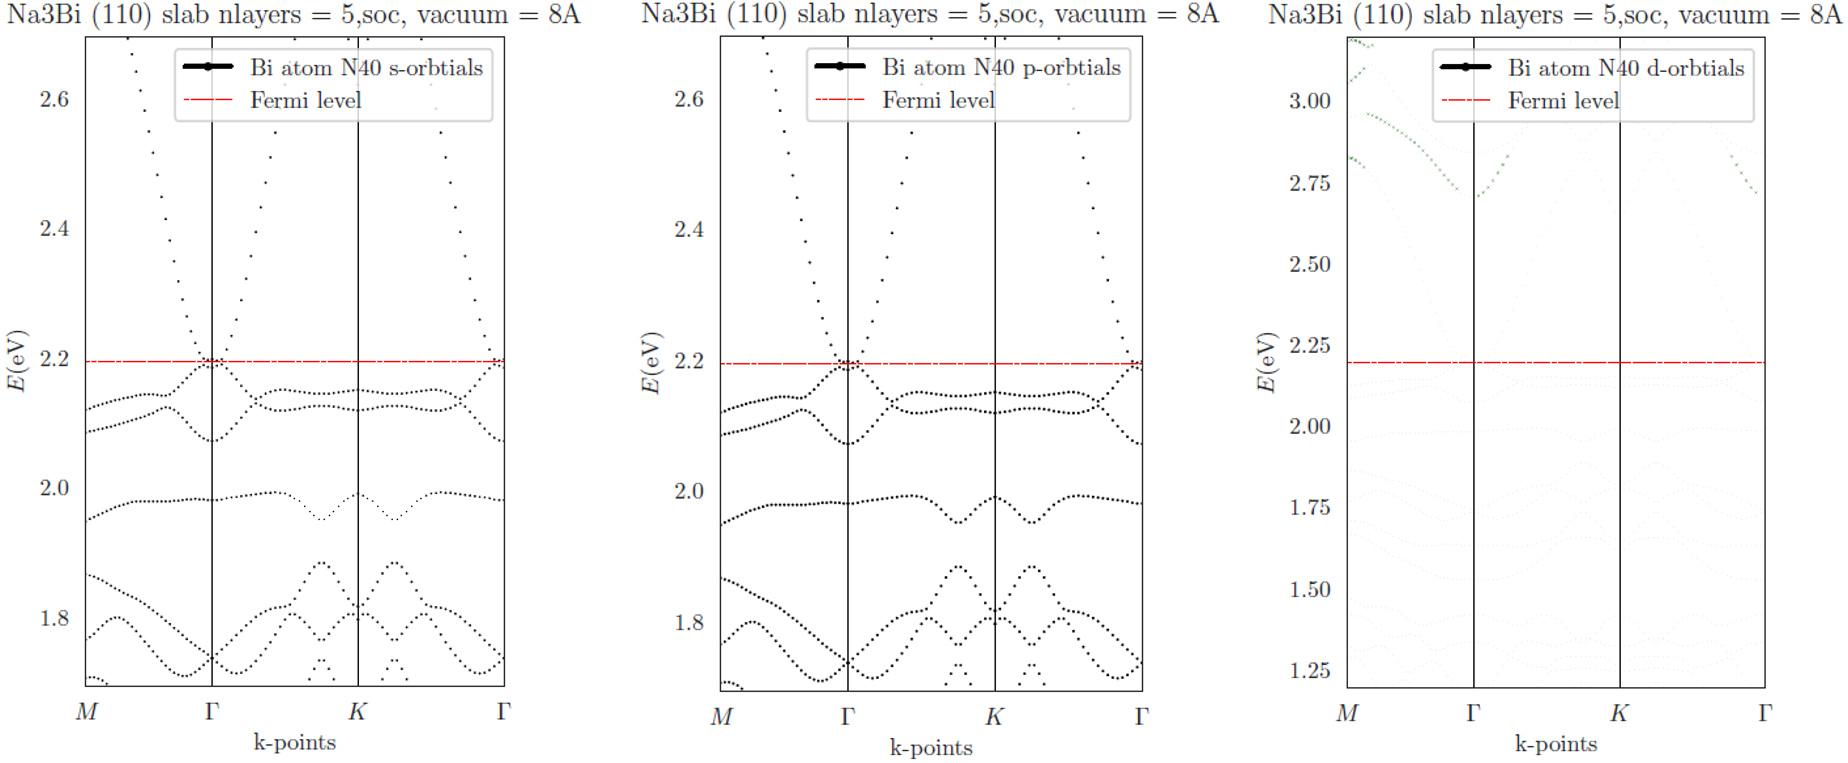
\includegraphics[scale=0.5]{Na3Bi_110_nlayer5_vac8_fatbands_Bi_N40}

\caption{\label{fig:Na3Bi_110_nlayer5_vac8_fatbands_Bi_N40} Fat band plots showing the contributions of Bismuth's orbitals on the band plot of 5 layer Na$_3$Bi in an 8A vacuum.}

\end{figure}


\begin{itemize}

\item In Figure \ref{fig:Na3Bi_110_nlayer5_vac8_fatbands_Bi_N40} we plot the contributions of Bismuth's on the band structure for Na$_{3}$Bi.  
\item The Bi atom, labeled as atom number 40,  is located on the top surface of the Na$_{3}$Bi slab. 
\item Bismuth's p-orbtials contribute the most to the band plot, followed by its s-orbitals. The d-orbitals contribute the least.
\end{itemize}


\begin{figure}[H]

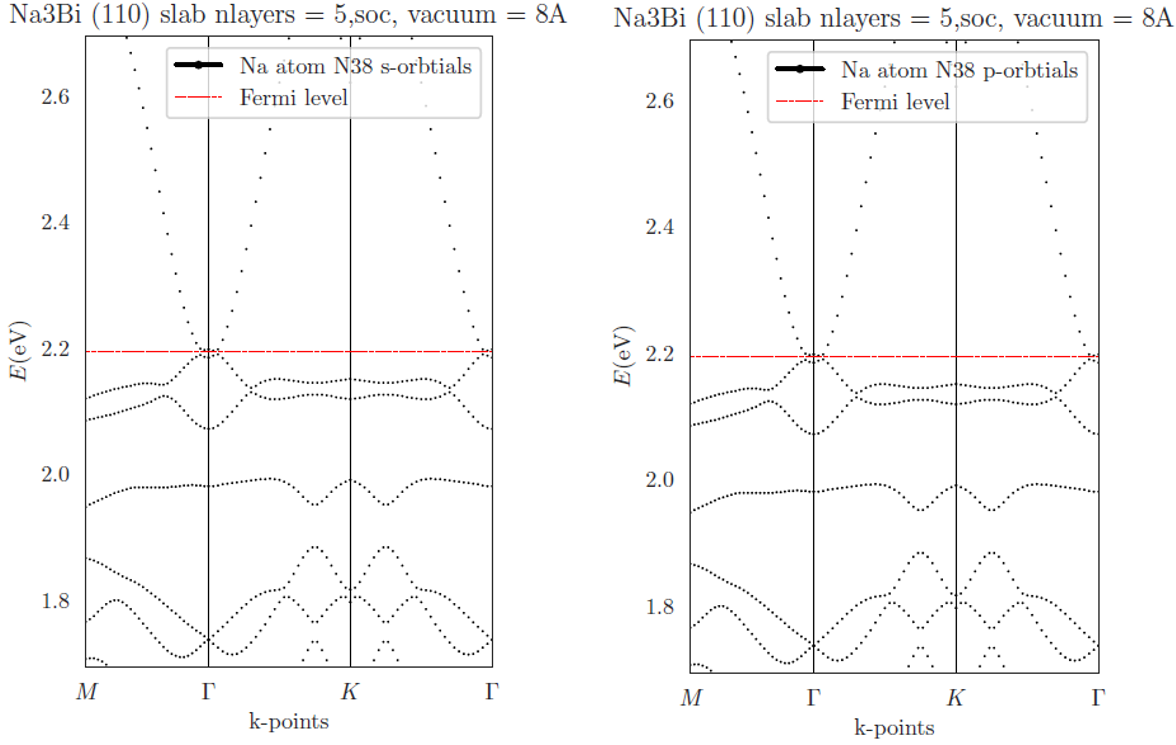
\includegraphics[scale=0.5]{Na3Bi_110_nlayer5_vac8_fatbands_Na38}

\caption{\label{fig:Na3Bi_110_nlayer5_vac8_fatbands_NaN38}The fat band plots of Sodium's orbitals on the band plots of 5 layer Na$_3$Bi in an 8A vacuum background.}

\end{figure}


\begin{itemize}

\item In Figure \ref{fig:Na3Bi_110_nlayer5_vac8_fatbands_NaN38} we plot the contributions of Sodium's s and p orbitals to Na$_3$Bi's band plot.  
\item This Na atom is on the top surface of the Na3Bi slab.  
\item It appears that both orbitals have equally relevant contributions to Na$_{3}$Bi's band plot.

\end{itemize}


%Aluminum on Na3Bi heterostructure.
\subsection{Aluminum on Na$_3$Bi heterostructure data.}

\begin{itemize}

\item We want to investigate the fate of the Na3Bi surface states when Na$_3$Bi layers are stacked on Aluminum (Al) layers. 
\item We want to answer whether any hybridization occurs between the Na$_3$Bi surface states and the Al metallic states. If so, does this produce topological states?
\item We also want to observe how far the spin texture characterizing the Na$_3$Bi surface states penetrate into the Al surface. 
\item Since Na$_3$Bi and Al have distinct crystal structures, the former has a hexagonal P63/mmc phase crystal structure while the latter has a face-centered cubic crystal structure, they need to be stacked along certain orientations to minimize the lattice mismatch between both structures. 
\item Based on information from the Materials Project website, we orientate Al along the (111) direction on Na$_3$Bi, which is along the (110) direction.

\end{itemize}

%Band structure plot and electronic density of states for 1Al/3_Na3Bi heterostructure. 
\begin{figure}[H]

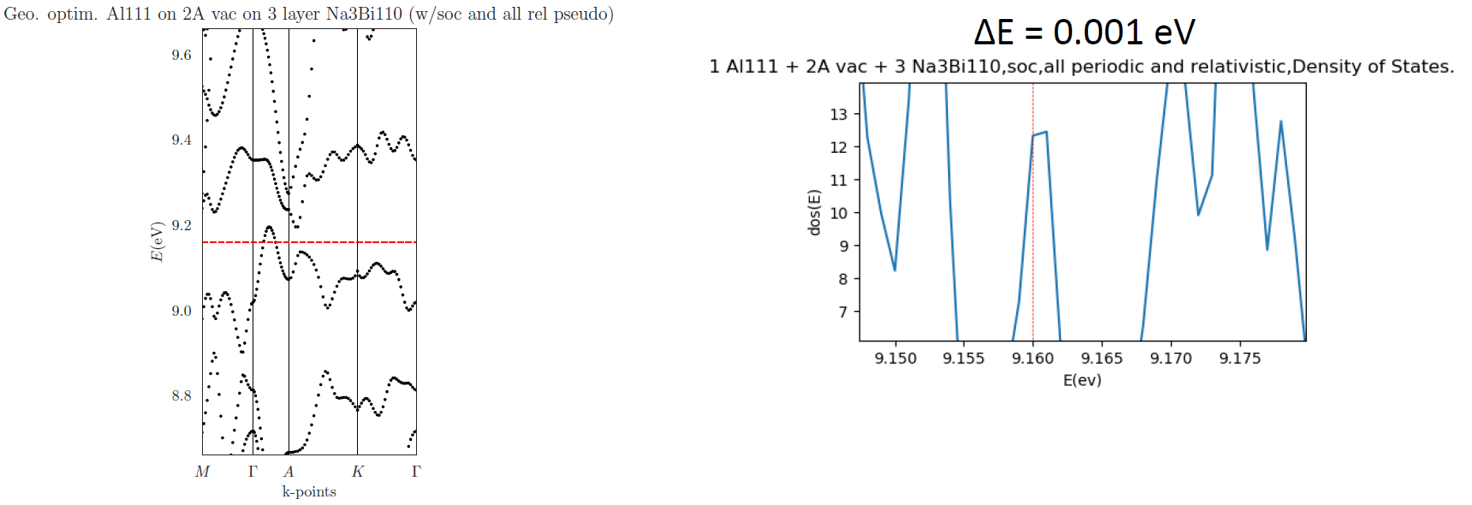
\includegraphics[scale=0.8]{Al111_on_Na3Bi_bandplot&DOS}\caption{\label{fig:1Al+3Na3Bi bandplot =000026 DOS.}Band structure plot and
electronic density of states for geometrically optimized Al/Na$_3$Bi heterostructure.}

\end{figure}


\begin{itemize}
\item We studied a single layer Al (111) on three layers of Na$_3$Bi (110) which were initially separated by 2A.  
\item We then perform a geometric relaxation calculation on this heterostructure.  It involves finding the optimal positions of the atoms in the heterostructure as well as the optimal cell of this structure.  
\item These optimizations are realized when the total energy and all components of the forces acting acting on all the atoms are below certain thresholds.
\item Figure \ref{fig:1Al+3Na3Bi bandplot =000026 DOS.} shows the band plot and electronic density of states for the geometrically relaxed heterostructure consisting of a single layer Al (111) on three layers of Na$_3$Bi (110).   
\item We observe this heterostructure is metallic since the Fermi level, indicated by the red dashed line, intersects a band with no finite energy gap immediately above the Fermi level which separates the filled and unfilled electronic states.
\item We find the same conclusion if we study the density of electronic states. This quantity signifies the number of available electronic states per unit energy per unit volume. We see above that there is a non-zero density of states around the Fermi level. 

\end{itemize}




%Modulus squared and modulus of wavefunctions of bands nearest the Fermi level at \Gamma. for the heterostructure. 
\begin{figure}[H]

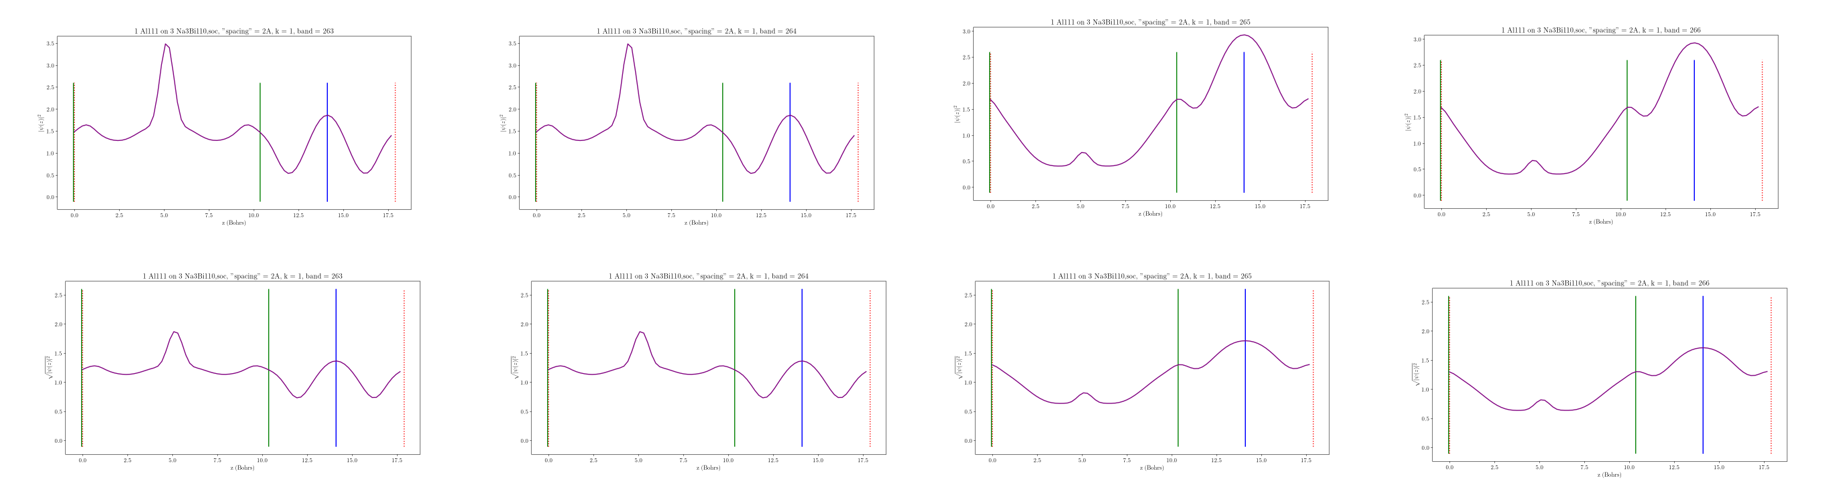
\includegraphics[scale=0.6]{Al111_on_Na3Bi_wavefunctions}\caption{\label{fig:Modulus squared and modulus of bands}Modulus squared and
modulus of bands closest to the Fermi level.}

\end{figure}



\begin{itemize}
\item Our heterostructure resides in $3+1$ dimensions.  The z-direction has open boundary conditions, while periodic boundary conditions are applied in the x and y directions.
\item Figure \ref{fig:Modulus squared and modulus of bands} shows the behavior of the modulus squared and modulus $\left|\psi\left(z\right)\right|^{2}$ and $\sqrt{\left|\psi\left(z\right)\right|^{2}}$ of the wavefunctions corresponding to bands $263 - 266$.  These are the the bands closest to the Fermi level at $\Gamma$. The valence bands correspond to bands 263 and 264, while the conduction bands are bands 265 and 266.
\item The green and blue vertical lines denote the boundaries of the Na$_3$Bi and Al layers, respectively, while the red dashed lines are the boundaries of the structure which includes any space between the Na$_3$Bi and Al layers.
\item The valence bands have a modulus that is peaked around the center of the Na$_3$Bi system. This modulus dips in the region between the Na$_3$Bi and Al layers and between the Al layers and the upper structure boundary.  
\item A relative maximum of the modulus that appears at the single Al layer.
\item The conduction bands' squared moduli behave completely different; their maxima appears around the Al layer.
\item Relative maxima in the squared moduli occur at the surfaces of the Na$_3$Bi structure.
Between the Na$_3$Bi and Al structure, the squared moduli are not at all minimum. 
\item Conduction bands have a minimum around the center of the Na$_3$Bi structure. 
\item As for the analogous moduli plots, there is not much to say for them: they appear to follow the trends of the modulus squared plots.
\item The moduli plots indicate there is no hybridization between the Na$_3$Bi surface states and the Al states. 
\item However, we only have a single Al layer present. We want to increase number of Al layers in the heterostructure to observe any changes in the modulus and modulus squared plots as well as the band plots.
\item Additionally, we are attempting to find the behavior of the surface states in a heterostructure consisting of Na$_3$Bi and KTaO$_3$, the latter being an insulator.
\end{itemize}


\end{document}
